\section{Distribución hipergeométrica}
\subsection{Muestreo sin reemplazo y fórmulas poblacionales}

La distribución hipergeométrica modela el número de éxitos en $n$ extracciones \emph{sin reemplazo} de una población finita de tamaño $N$ que contiene $K$ éxitos y $N-K$ fracasos. Su función de probabilidad es
\begin{align}
 \label{eq:2.10.11}
 f(k) = P(X=k) = \dfrac{\binom{K}{k}\binom{N-K}{n-k}}{\binom{N}{n}}, \quad \max(0, n-(N-K)) \leq k \leq \min(n, K).
\end{align}

A diferencia de las distribuciones anteriores, los ensayos aquí \emph{no son independientes} porque el muestreo sin reemplazo altera las probabilidades en cada extracción.

{Propiedades de la distribución hipergeométrica} Si $X$ tiene distribución hipergeométrica con parámetros $N$, $K$ y $n$, entonces
\begin{align}
 \mu_{X} &= n\dfrac{K}{N} \\
 \s_{X}^{2} &= n\dfrac{K}{N}\dfrac{N-K}{N}\dfrac{N-n}{N-1}.
\end{align}

El factor $\dfrac{N-n}{N-1}$ se conoce como \emph{factor de corrección por población finita}. Cuando $n \ll N$, este factor tiende a $1$ y la distribución hipergeométrica se aproxima a la binomial con parámetros $n$ y $p=K/N$.

\begin{ejemplo}
 \label{exmp:2.10.16}
 Un lote contiene $20$ piezas, de las cuales $5$ son defectuosas. Si se eligen $4$ piezas al azar sin reemplazo, ¿cuál es la probabilidad de encontrar exactamente $2$ defectuosas?
\end{ejemplo}

\begin{solucion}
	Aquí $N=20$, $K=5$, $n=4$, $k=2$.
	\begin{align}
		P(X=2) &= \dfrac{\binom{5}{2}\binom{15}{2}}{\binom{20}{4}} \\
		&= \dfrac{10 \times 105}{4845} \\
		&= \dfrac{1050}{4845} \approx 0.2167
	\end{align}
\end{solucion}

\begin{ejemplo}
 \label{exmp:2.10.17}
 En una mano de póker de $5$ cartas de una baraja de $52$, ¿cuál es la probabilidad de obtener exactamente $3$ reyes?
\end{ejemplo}

\begin{solucion}
	Aquí $N=52$ (total de cartas), $K=4$ (reyes), $n=5$ (cartas en la mano), $k=3$.
	\begin{align}
		P(X=3) &= \dfrac{\binom{4}{3}\binom{48}{2}}{\binom{52}{5}} \\
		&= \dfrac{4 \times 1128}{2598960} \\
		&= \dfrac{4512}{2598960} \approx 0.00174
	\end{align}
\end{solucion}

\lstinputlisting[language=Python]{../code/distribuciones-especiales/distHyper.py}

\begin{figure}
 \centering
 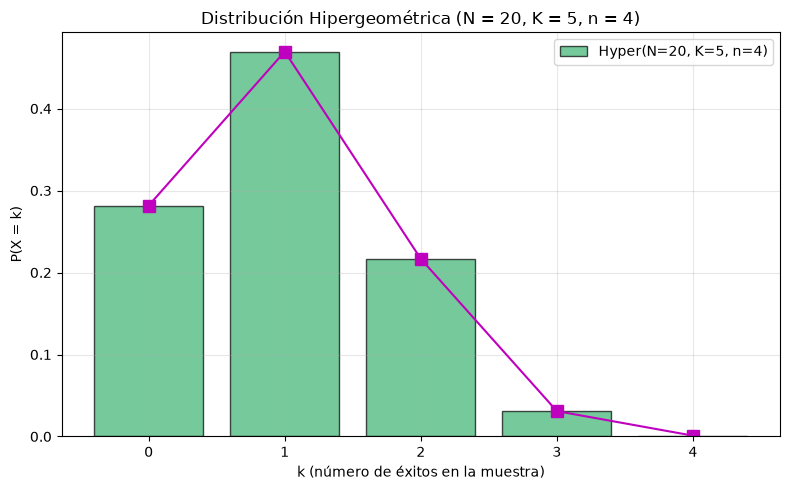
\includegraphics[height=7cm,keepaspectratio=true]{./pe/distHyper.png}
 % distHyper.png: 0x0 pixel, 300dpi, 0.00x0.00 cm, bb=
 \caption{Distribución hipergeométrica con $N=20$, $K=5$, $n=4$}
 \label{fig:2.10.9}
\end{figure}

\begin{observacion}
	La distribución hipergeométrica se reduce a la binomial cuando el muestreo es con reemplazo (o equivalentemente, cuando $N \to \infty$). En la práctica, si $\frac{n}{N} < 0.05$, la aproximación binomial es razonablemente precisa.
\end{observacion}


